\documentclass[twocolumn,onesided,9pt]{article}

\usepackage{./Task32FlyerLatexStyle/Task32Flyer}
\usepackage{todonotes}

%% -----------------------------------
%% Document information
%% -----------------------------------
\def\pubdate{DRAFT 02 April 2020}
\title{Status Update: IEA Wind Recommended Practice 15 on Ground-Based Vertically-Profiling Remote Sensing For Wind Resource Assessment (2013)}
\shorttitle{Status update: RP15}
\DOI{10.5281/zenodo.xxxxxx}
\addbibresource{bibliography.bib}

%% ===================================
%% Document - specific commands
%% ===================================
\usepackage[export]{adjustbox}
\newcommand{\RP}[1]{RP #1}
\newcommand{\note}[1]{RP #1}
\newcommand{\RPdetails}[2]{\textbf{\RP{#1}:\ #2.}}

%% ===================================
%% Document starts
%% ===================================
\begin{document}
	
	%% -----------------------------------
	%% Title
	%% -----------------------------------
	\maketitle
	\thispagestyle{cover}
	
	%% -----------------------------------
	%% Introductory text
	%% -----------------------------------
	{\Large\noindent%
		IEA Wind published recommended practices on ground-based remote sensing in 2013. Is it valid in 2020?
	}
	\vskip 6pt
	
	Recommended Practices don't have an expiry date, but they can become outdated. In this status update we provide our perspective on how developments in wind lidar technology since 2013 impact the IEA Wind Recommended Practice 15 on Ground-Based Vertically-Profiling Remote Sensing For Wind Resource Assessment.
	
	%% -----------------------------------
	%% About
	%% ----------------------------------- 
	\section*{The 2013 Recommended Practices}
	
	The 2013 Recommended Practices document was developed by the wind lidar and sodar community in response to a clear need for a document that would establish repeatable good practice in measurements with active remote sensing devices (RSDs).
	
	As was noted in the preface to the document,
	
	\begin{quotation}
	
The purpose of this recommended practice is to document the steps required to collect high-quality, well-documented remote sensing data for use in wind resource assessments on land. 

	\end{quotation}
		
	The document provided specific guidance as ``Recommended Practices'' (e.g., RP1) and informative notes (e.g. Note 1) about how to use remote sensing. There were 41 RPs and 22 notes in total, covering many different aspects of the remote sensing lifecycle.
	
	These RPs represented the community's perceptions of how to do things, and were not always based on evidence. Thus the 2013 document was a ``recommended practice'', not a standard. Since 2013 there have been several standards and other documents adopted that may supersede some RPs from 2013.
	
	The 2013 Recommended Practices document can be downloaded from the \href{https://community.ieawind.org/task32/ourlibrary/publications}{IEA Wind Task 32 website} or the \href{https://github.com/IEA-Wind-Task-32/RP15-Ground-Based-Remote-Sensing-for-Wind-Resource-Assessment/releases/tag/1.0}{IEA Wind Task 32 GitHub repository}.
	
	\begin{figure}[h]
		\centering
		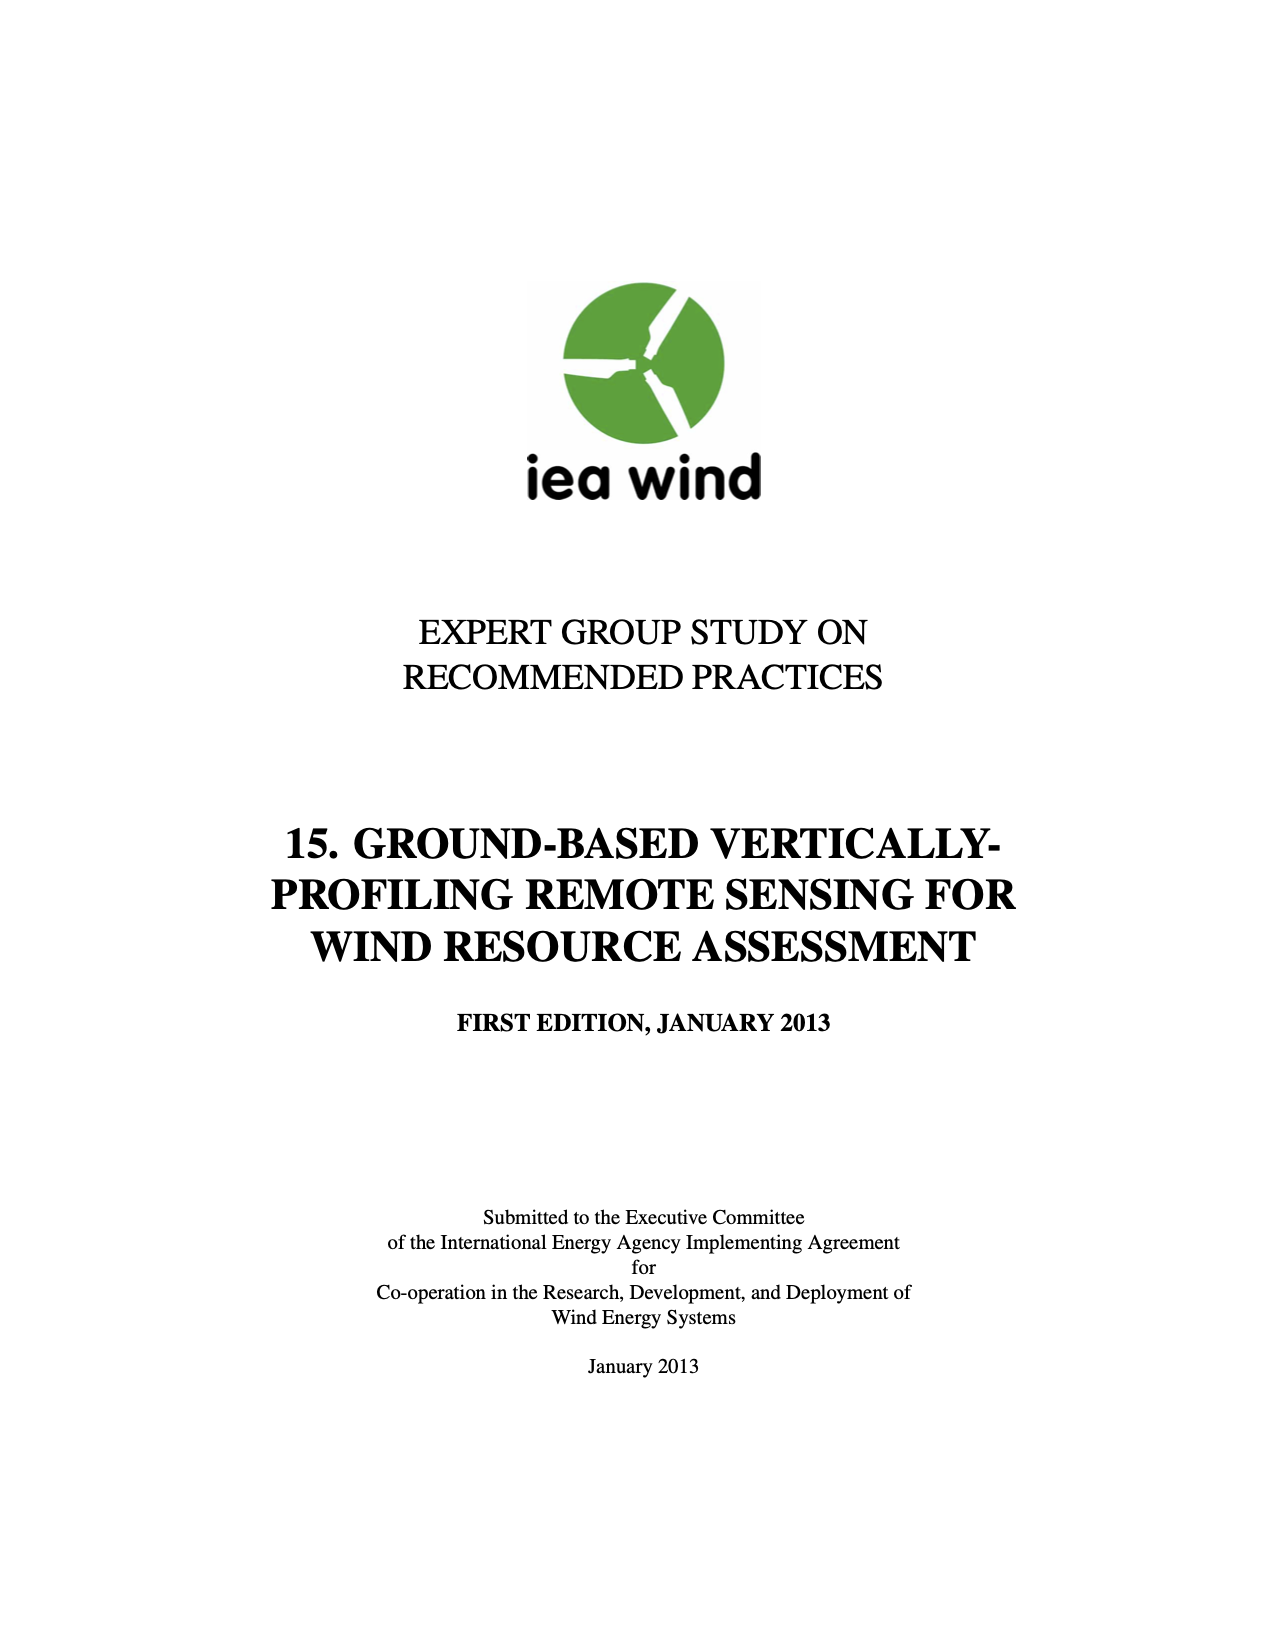
\includegraphics[width=0.9\linewidth, frame]{graphics/RP2013.png} 
		\caption{The 2013 Recommended Practices}
		\label{fig:RP2013}
	\end{figure}	
	
	
	\section*{Scope of this document}
	
The 2013 document was ``designed to guide the use of ground-based, fixed scan geometry, vertically-profiling wind remote sensing using lidar and sodar for the resource assessment phase of an on-shore wind farm development. Lidar and sodar that use these methods are referred to generically in the document as remote sensing devices, or RSD.''
	
	This update provides guidance on the relevance of the RPs from 2013 to \textbf{ground-based wind lidar devices being used for the same applications in 2020}.

	%% -----------------------------------
	%% Feedback
	%% ----------------------------------- 	
	
	\section*{Feedback}
	Feedback about the 2013 Recommended Practices document should be made via the \href{https://github.com/IEA-Wind-Task-32/RP15-Ground-Based-Remote-Sensing-for-Wind-Resource-Assessment/issues}{GitHub repository}.
	
	Feedback about this status update should be directed to the \href{https://github.com/IEA-Wind-Task-32/RP15-Ground-Based-Remote-Sensing-for-Wind-Resource-Assessment}{Task 32 Operating agents}.
	
	
	\section*{Relevance of the 2013 Recommended Practices in 2020} 
	
	Following is a review of the 2013 Recommended Practices referencing the section numbers (e.g., \S 2.3) and individual recommended practices (e.g. \RP{1}) in that document.
	%% -----------------------------------
	%% Characterizing RSD (RP1)
	%% ----------------------------------- 

	\subsection*{\S 2 Characterizing remote sensing devices}
	A remote sensing device should be appropriately characterized. The important characteristics of a wind lidar are the same in 2020 as in 2013.

	\RPdetails{1}{Documentation of RSD characteristics} Still relevant.
	 
	%% -----------------------------------
	%% Installing RSD (RP2-16)
	%% ----------------------------------- 

	 \subsection*{\S 3 Installing remote sensing devices}
	 \subsubsection*{\S 3.1 Training}
	 The 2013 document described the need to provide and document training. This is still important to get the best data from a wind lidar or any other measurement sensor.
	 
	 \RPdetails{2}{Training of workers} Still relevant.

	 \subsubsection*{\S 3.2 Site selection}
	 \RP{3} in the 2013 document addressed the issue of flow homogeneity, and suggested deploying RSD away from regions of heterogeneous flow.
	 
	 There are now many commercially-available tools and services that address the effect of flow homogeneity on RSDs and aim to make RSD data comparable to a point measurement (e.g. from a cup anemometer). This may make it possible to use RSDs in more heteorogeneous flows than was considered appropriate in 2013. However, the need to be aware of flow hetereogeneity and respond appropriately has not changed.
	 
	 \RPdetails{3}{Deployment in complex flow environments} Still relevant.
	 
	 An IEA Wind Task 32 working group on wind lidar complex terrain is carrying out a group study on several different tools to support the use of wind lidar in complex terrain. Results are expected in 2021 and may lead to the publication of guidelines for this use case.
	
	\subsubsection*{\S 3.3 Transport}
	Any piece of wind measurement equipment should be transported appropriately.

	\RPdetails{4}{Reusable protective packaging for RSD transport} Still relevant.
	
	\RPdetails{5}{Installation of shock detectors on the RSD} Still relevant.
	
	\subsubsection*{\S 3.4 Site preparation}
	\RP{6} in the 2013 document was intended to ensure that the RSD had ``...a clear view of the sky that was largely free of obstructions.'' This is still recommended.
	
	\RPdetails{6 a,b}{Site reconnaissance, clearing and structures} Still relevant.
	
	Since 2013, wind lidar devices and the associated data processing tools have become better able to deal with obstructions or small-scale inhomogeneity, and thus it is no longer recommended to avoid tower or structure wakes, or deployments where part of the lidar scan pattern is obstructed.
	
	\RPdetails{6 c,d}{Measurements in tower or structure wakes, avoiding beams interacting with structures} Deprecated.
	
	\subsubsection*{\S 3.5 Orientation}
	\RP{7} aimed at reducing or eliminating installation accuracy concerns.
	
	\RPdetails{7}{Device alignment} Still relevant.
	
	\subsubsection*{\S 3.6 Tilt and roll}
	\RP{8} and \RP{9} aimed at reducing or eliminating the effect of device alignment on the measurements, and detecting gradual settling
	
	\RPdetails{8a}{Device coarse leveling} Still relevant.

	\RPdetails{8b}{Device fine leveling} may be mitigated by the lidar's own ability to compensate for small tilt or roll.
	
	\RPdetails{9}{Tilt sensors on the RSD} Still relevant, but small settling angles may be mitigated by \RP{8b}.
	
	\subsubsection*{\S 3.7 Time snychronization}
	The 2013 Recommended Practice document suggested the use of an accurate external time reference. This is still important when using data from the lidar.
	
	\RPdetails{10}{Time sychronization} Still relevant.
	
	\subsubsection*{\S 3.8 Power supply}
	As in 2013, remote wind lidar often still require stand-alone power systems, and care should be taken in sourcing and fuelling these power systems. However, compared to 2013, there are now many more experienced service providers who are able to support remote wind lidar deployments.
	
	\RPdetails{11}{Design of remote power systems} Still relevant.

	\RPdetails{12}{Fueled remote power systems} Still relevant.

	\subsubsection*{\S 3.9 Protection from interference}
	Like any unattended equipment, care should be taken to protect a ground-based lidar from interference.

	\RPdetails{13}{Protection from interference} Still relevant.
	
	\subsubsection*{\S 3.10 Safety signs and interlocks}
	Properly operated and maintained remote sensing devices should pose no hazard to the public, outside of the enclosure.

	\RPdetails{14}{safety signs, interlocks and operation} Still relevant.

	\subsubsection*{\S 3.11 Function check}
	An extensive set of functional tests were suggested for the RSD to show that the RSD was properly working before being left unattended. These are still important, but might be implemented as part of automated tests at power-up by the RSD.
		
	\RPdetails{15}{Function checklist} Still relevant.
	
	\subsubsection*{\S 3.12 Installation report}
	The 2013 document proposed an extensive installation report. This was intended to be the basis for third-party reporting.
	
	\RPdetails{16}{Installation report} Still relevant, but possibly superseded by installer's report formats.
	
	%% -----------------------------------
	%% Operating RSD (RP17-24)
	%% ----------------------------------- 

	\subsection*{\S 4 Operating remote sensing devices}

	\subsubsection*{\S 4.1 Communications}
	The 2013 Recommended Practices proposed how remote access to the RSD could be provided and what might be done. These capabilities are still required today.
	
	\RPdetails{17}{Remote access to the RSD} Still relevant.
	
	\subsubsection*{Sensitivity to ambient conditions}
	In 2013, wind lidar were still relatively new devices and there was a lack of consensus about their behaviour in different weather conditions. \RP{18} and \RP{19} recommended that measures should be taken to document and if possible, mitigate the effects of ambient conditions on the RSD.
	
	These recommendations have since been superseded by the development of ambient condition sensitivity tests for RSDs as part of the 2017 revision of the IEC 61400-12-12 standards for power performance verification of wind turbines.
	
	\RPdetails{18}{Lidar fog and cloud detection} Deprecated. Superseded by IEC 61400-12-1 (2017) \cite{IEC_61400_12_1_2017}.
	
	\RPdetails{19}{Mitigation of precipitation effects on measurements} Deprecated. Superseded by IEC 61400-12-1 (2017) \cite{IEC_61400_12_1_2017}.
	
	\RP{20} and \RP{21} are not relevant to wind lidar.
	
	\subsubsection*{\S 4.3 Local weather conditions}
	\RP{22} recommended the installation of weather sensing data to understand the RSD performance and assist in predicting AEP. This information is still useful, but can be linked to the results of a sensitivity assessment according to IEC 61400-12-1 (2017) \cite{IEC_61400_12_1_2017}.
	
	\RPdetails{22}{Monitoring weather conditions} Still relevant. Should include any sensitivity effects identified according to IEC 61400-12-1 (2017) \cite{IEC_61400_12_1_2017}.
	
	\subsubsection*{\S 4.4 Servicing and maintenance}
	RSD may require maintenance from time to time, and this may result in some impact on the RSD measurements. \RP{23} recommended that the user and RSD supplier to work together to ensure reliability and repeatability, and is still applicable to wind lidar.
	
	\RPdetails{23}{Recommended service intervals} Still relevant.
	
	\subsubsection*{\S 4.5 Operation and maintenance log}
	\RP{24} recommended the user keep a log of all use and maintenance of the RSD. Experience has shown that a log can be very valuable.

	\RPdetails{24}{Operation and maintenance log} Still relevant.
	
	%% -----------------------------------
	%% Remote sensing data analysis (RP 25-29)
	%% ----------------------------------- 

	\subsection*{\S 5 Remote sensing data analysis}

	\subsubsection*{\S 5.1 Wind speed and vector}
	\RP{25}, 26 and 27 recommended storing data at several points during RSD data processing. These steps are still required for wind lidar.
	
	\RPdetails{25}{Line-of-sight wind velocity} Still relevant.
	
	\RPdetails{26 a, b}{Instantaneous wind vector} Still relevant.
	
	\RPdetails{26 a, c}{Instantaneous wind vector} Deprecated. This can be derived from the data stored under \RP{26 a} and \RP{26 b}.
	
	\RPdetails{27}{Time-averaged wind vector} Still relevant.
	
	\subsubsection*{\S 5.2 Turbulence intensity}
	In 2013, \RP{28} noted that `the ability to generate or report an estimate of the turbulence intensity is not required but may be advantageous for some applications'. 
	
	Since then, there has been much research into the ability of wind lidar to measure wind turbulence \citep[see e.g.,][]{clifton_2018_a}. The consensus in the wind lidar community is that the wind turbulence derived by a wind lidar is not the same as measured by a cup anemometer, but there may be ways to adjust the two values so that they agree.
	
	The effectiveness of several tools to adjust wind lidar turbulence data will be investigated by the Consortium for the Advancement of Remote Sensing (CFARS, \href{http:\\www.cfars.org}{www.cfars.org)} in 2020.
	
	For those reasons, \RP{28} should be considered deprecated, pending an update from CFARS.
	
	\RPdetails{28}{Derivation of turbulence intensity} Deprecated.
	
	\subsection*{\S 5.3 Extreme gusts}
	\RP{29} suggested that extreme gust information derived from RSD data could be used if required, and that verification data would also be required.
	
	\todo[inline]{not sure what the case is here in 2020}
	
	\subsection*{\S 5.4 Correcting for errors due to flow inhomogeneity}
	Section 5.4 and \note{17} noted that flow inhomogeneity may introduce differences between RSD and cup anemometers. As was noted in the discussion of \RP{3}, this is the subject of ongoing community research and results are expected in 2021.

	%% -----------------------------------
	%% Verification of remote sensing devices (RP 30 - 41)
	%% ----------------------------------- 
	
	\subsection*{\S6 Verification of remote sensing devices}
	Section 6 of the 2013 Recommended Practices document includes recommendations about how to test the performance of a remote sensing device, quantify it, estimate uncertainty, and how to document it. These RPs (RP 30 - 40, inclusive) have all been superseded by the publication of the IEC 61400-12-1 (2017) standard \cite{IEC_61400_12_1_2017}.
	
	\RPdetails{30}{Verification of wind speed and direction} Deprecated. Superseded by IEC 61400-12-1 (2017) \cite{IEC_61400_12_1_2017}.

	\RPdetails{31}{Verification of turbulence intensity} Deprecated. Superseded by IEC 61400-12-1 (2017) \cite{IEC_61400_12_1_2017}.

	\RPdetails{32}{Comparisons at multiple heights with respect to the proposed turbine} Deprecated. Superseded by IEC 61400-12-1 (2017) \cite{IEC_61400_12_1_2017}.

	\RPdetails{33}{Verification dataset} Deprecated. Superseded by IEC 61400-12-1 (2017) \cite{IEC_61400_12_1_2017}.

	\RPdetails{34}{Preparation of verification dataset} Deprecated. Superseded by IEC 61400-12-1 (2017) \cite{IEC_61400_12_1_2017}.

	\RPdetails{35}{Document the reference dataset} Deprecated. Superseded by IEC 61400-12-1 (2017) \cite{IEC_61400_12_1_2017}.

	\RPdetails{36}{Demonstrating clock synchronization with reference devices} Deprecated. Superseded by IEC 61400-12-1 (2017) \cite{IEC_61400_12_1_2017}.

	\RPdetails{37}{Reporting of verification results} Deprecated. Superseded by IEC 61400-12-1 (2017) \cite{IEC_61400_12_1_2017}.

	\RPdetails{38}{Reporting of RSD verification relationship to flow conditions} Deprecated. Superseded by IEC 61400-12-1 (2017) \cite{IEC_61400_12_1_2017}.

	\RPdetails{39}{Uncertainty estimate} Deprecated. Superseded by IEC 61400-12-1 (2017) \cite{IEC_61400_12_1_2017}.

	\RPdetails{40}{Verification report} Deprecated. Superseded by IEC 61400-12-1 (2017) \cite{IEC_61400_12_1_2017}.

	\RPdetails{41}{Periodic device verification} Deprecated. Superseded by IEC 61400-12-1 (2017) \cite{IEC_61400_12_1_2017}.
	
	
	\section*{Summary}
	Many of the 2013 IEA Wind Recommended Practice 15 on Ground-Based Vertically-Profiling Remote Sensing For Wind Resource Assessment are still relevant in 2020, particularly in relation to general good practice when deploying, operating, and maintaining wind lidar.
	
	However, almost all verification activities have been superseded by the publication in 2017 of the IEC 61400-12-1 Standard for power performance measurements \cite{IEC_61400_12_1_2017}. It is our expectation that the development of a new family of IEC standards for instrumentation and measurements in the 2020's may in turn deprecate the IEC 61400-12-1 standard.	
		
	%% -----------------------------------
    %% References
    %% -----------------------------------
    %\subsection*{References}
    % bibliography
    \label{sec:References}
    \addcontentsline{toc}{section}{References}
    {\small
    \printbibliography
    }
	\vspace*{\fill}

	%% -----------------------------------
	%% Outlined block of smaller text
	%% -----------------------------------
	\begin{tcolorbox}[width=1.0\columnwidth,
		boxsep=0pt,
		left=3pt,
		right=3pt,
		top=3pt,
		arc=0pt,
		boxrule=0.5pt,
		toprule=0.5pt,
		colback=white,
		coltext=TextGrey
		]
		{\footnotesize
			This document was self published by IEA Wind Task 32.
			
			%% -----------------------------------
			%% IEA WIND AND TASK 32
			%% -----------------------------------
			\begin{tabular}{m{0.3\columnwidth}m{0.6\columnwidth}}
				% IEA Wind * DO NOT EDIT THIS TEXT *
				
\includegraphics[height=2cm]{graphics/IEAWind_logo.jpg} &
				The International Energy Agency is an autonomous organisation which works to ensure reliable, affordable and clean energy for its 30 member countries and beyond. The IEA Wind Technology Collaboration Programme supports the work of 38 independent, international groups of experts that enable governments and industries from around the world to lead programmes and projects on a wide range of energy technologies and related issues.%
				\\
				% Task 32 * DO NOT EDIT THIS TEXT *
				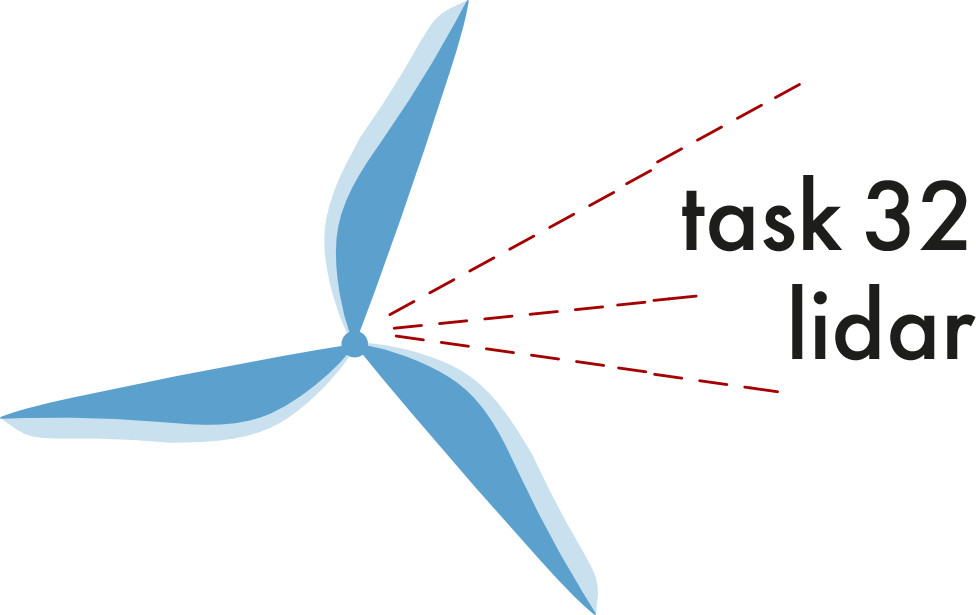
\includegraphics[height=1.5cm]{graphics/Task32_logo.jpg} &
				\href{https://community.ieawind.org/task32/home}{IEA Wind Task 32} exists to identify and mitigate the barriers to the deployment of wind lidar for wind energy applications.
			\end{tabular}%
			
			%% -----------------------------------
			%% For more information
			%% -----------------------------------
			% N.B. do not add line breaks between the next items
			\textbf{For more information:} See the  \href{https://community.ieawind.org/task32/home}{Task 32 website}.
			%% -----------------------------------
			%% Authors
			%% -----------------------------------
			\textbf{Author team:} %
			Andrew Clifton (Task 32 Operating Agent, University of Stuttgart, Germany), %
			xxx (org x), 
			yyy (org y).
			%% -----------------------------------
			%% Reviewers
			%% -----------------------------------
			%\textbf{Reviewers:} %
			% first last (short affiliation), %
			% first last (short affiliation).
			%% -----------------------------------
			%% Images
			%% -----------------------------------
			\textbf{Images:}
			Banner, left to right: \href{https://unsplash.com/@alexkixa}{Alexandre Debiève on Unsplash}, \href{http://ifb.uni-stuttgart.de}{SWE U. Stuttgart}, \href{https://unsplash.com/@markusspiske}{Markus Spiske on Unsplash}.
		}
		
		%% -----------------------------------
		%% End of highlighted block
		%% -----------------------------------
	\end{tcolorbox}
	\vspace*{\fill}

\end{document}
